% Chapter Template

\chapter{Reconstructing networks from statistical distributions} % Main
% chapter title

\label{Chapter-Reconstruction} % Change X to a consecutive number; for
% referencing this chapter elsewhere, use \ref{ChapterX}

\lhead{Chapter 5. \emph{Reconstructing the Network from Statistical
Distributions}} % Change X to a consecutive number; this is for the header on each page - perhaps a shortened title

%----------------------------------------------------------------------------------------
%	SECTION 1
%----------------------------------------------------------------------------------------

\section{Methods}

The software used in this chapter, has been independently developed here, but is based on the
idea of \citet{lindstrom_biopolymer_2010} about reconstructing the network
architecture of polymers networks from a statistical description. They were
based on the work of \citet{yeong_reconstructing_1998,yeong_reconstructing_1998-1}
about reconstructing random porous media.\\
The input for the in-silico reconstruction of biopolymer networks is the
statistical distributions of $3$ properties in this case. This is the minimal
set of information required to reconstruct the architecture of the network to study the
mechanical properties (but other parameters could be added to study other or
more complex situations). For example, if the structure of the edges / chains is
heterogeneous  (bio-functional areas, or different charge distribution), extra
statistical distributions can be added with minimal effort.

So in order to regenerate the network in-silico, the following distributions
should be obtained from the image analysis:
\begin{figure}[h!]
\begin{center}
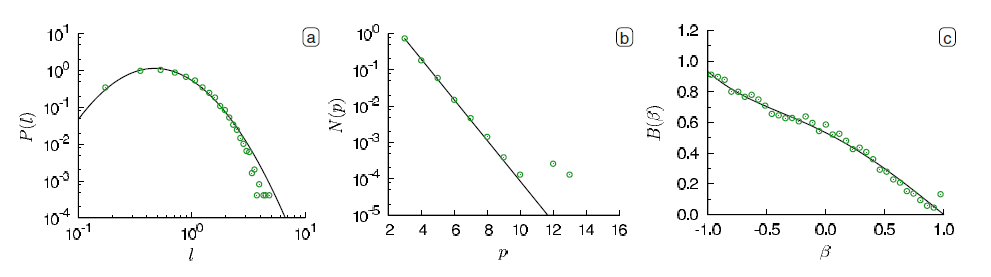
\includegraphics[width=1.0\textwidth]{Figures/chapter-reconstruct/lindstrom-paper-images.png}

\caption[Collagen distributions]{Collagen I distributions proposed by Lindstrom
\citep{lindstrom_biopolymer_2010}}

\end{center}
\end{figure}

\begin{enumerate}
\item \textbf{Degree of nodes $N(p)$.} i.e. number of edges per node
or cross-link.
\item \textbf{Length of edges $P(\ell$).} Length of the edges
between connected nodes.
There are two options to define this length.
\begin{itemize}
\item End to end vector distance (EtE-length). Consider the edge as a straight
line between nodes.

\item Contour length (curved). Take into account all the path of the chain,
usually curved.
\end{itemize}

In fact for many examples the difference between these is less than one
might have expected at a first glance. \citet{nisslert_identification_2007},
who use a different reconstructing algorithm, report that straight and curved
lengths have similar distribution, although the straight lines were about a
$15\%$ shorter.\\
I expect that high flexibility of chains and/or low density of cross-links
would increase the differences between them. Biopolymers tend to be semi-flexible, stiff
enough to keep this difference low.
The difference between these lengths can be used as a measure of the
persistence length (\gls{Lp}) of the chains.


\item \textbf{Direction cosine $B(\beta$)} between incident edges. Takes into
account the relative orientation of the edges incident on the same node.


\end{enumerate}

As described in this thesis, these distributions can be obtained using \textbf{image analysis} of data from
\gls{confocal}, or transmission electron microscopy (\gls{TEM}). See chapter \ref{Chapter-Image} for
more information about this.

The distributions used herein to develop the reconstruction software are those seen originally in
Lindstrom's paper \citep{lindstrom_biopolymer_2010}. These
distributions were selected because they fitted the data taken from image analysis of collagen I, but
no claim about their use in other systems was made.
% It is worth noting that I have noticed differences comparing
% the collagen distribution proposed here with our data in actin networks. The
% direction cosines distribution has a lot of variability, and it seems to
% follow a different distribution, however the degree and length distribution
% have similar shape in both systems.

It is worth reiterating that with the work described in this thesis, experimentally obtained distributions
describing the architectures of biopolymer networks can be extracted. Whatever functional forms are found to
faithfully represent the experimental data can be used to reconstruct in-silico networks. However, given the
similarities in the distributions we have found in \autoref{Chapter-Image} for very different biopolymer networks
we chose here to demonstrate the reconstruction using the following:


\begin{enumerate}
\item \textbf{$N(p)$}. The \textbf{node degree} modelled with a shifted geometric
distribution.

\begin{equation} \label{degree-dist}
N(p)=q(1-q)^{p-3}
\end{equation}
where $q=1/(Z-2)$, $p$ is the degree of the node - how many other nodes it is directly connected to - and Z is the average node degree.

The distribution is shifted because the minimum degree of a node is
$p=3$. The case $p=1$ corresponds to dead-ends nodes, and $p=2$ correspond to
bending nodes. We can ignore dead-ends because they don't affect to the mechanical properties of the bulk network. And the bending nodes
can be ignored if their $2$ edges are merged into a unique, larger edge,
connecting the neighbors of this bending node between them. Some information is lost in this
process if we are characterizing the length of edges by end to end
vectors.

\item \textbf{$P(\ell)$} The \textbf{length distribution} modelled as a
logarithmic-normal distribution.
\begin{equation} \label{length-dist}
P(\ell)=\frac{1}{\ell
s\sqrt{2\pi}}\exp{\bigg[-\frac{(\mu-\ln{\ell})^2}{2s^2}\bigg]}
\end{equation}
where $\mu$ and s are the mean and standard deviation of $\ln{\ell}$
respectively.
A gamma distribution \( P(\ell) = \frac{\ell^{\alpha - 1}\exp(-\ell/\beta)}{\Gamma(\alpha)\beta^\alpha} \) is also feasible to describe the lengths. We prefer the log-normal because it fits better in most cases and its two parameters
relate directly with computable network parameters.

%CHECK THAT LINDSTROM SAYS THAT \ell is normalized by n^{-1/3}
\item \textbf{$B(\beta)$} The \textbf{direction cosines distribution} has been modelled by
  a truncated power series.
\begin{equation} \label{cosines-dist}
B(\beta)=\sum_{k=1}^{m} b_k(1-\beta)^{2k-1}
\end{equation}
If we truncate it at $m=3$, and $B(\beta)$ is normalized to unity, then there
are two parameters left, $b_1$ and $b_2$ (or other combination).
\end{enumerate}

These $3$ distributions are enough to approximate the architecture of a
network of collagen if we are interested in its mechanical properties.
So, the network can be reconstructed with five
independent parameters:
$\mu$, s, $Z$, $b_1$ and $b_2$.


The output of the algorithm constructed is a network or spatial \gls{graph}, which is formed
by $2$ sets: a set of nodes, containing the nodes
position and the degree; and a second set of edges, which connect pair of
nodes. The software
does not allow parallel edges, i.e. two edges connected the same pair of nodes,
and the network is fully connected, there are no nodes or clusters of nodes
isolated  from the rest of the network.
%Not allowing parallel edges could be
%unrealistic in some situations, to deal with that, edges could be characterized
%by a thickness parameter, this parameter could be associated to the number of
%parallel edges merging in that edge.
\section{Euclidean Graph Generation Algorithm}
The Euclidean graph generation (EGG) algorithm reconstructs a $3D$
network on a periodic cube domain $\Sigma$ of size $\Lambda$. The algorithm uses
a Monte Carlo method with Simulated annealing, this is a general heuristic
method for global optimization which avoids the convergence to local minimums on
the energy landscape.

The following steps describe the algorithm:
\begin{enumerate}[label=\textbf{\Roman*}]
  \item An \textbf{initial graph configuration $H_0$} is generated by placing
  nodes drawn from a randomly uniform distribution inside the domain $\Sigma$. Then a
  valency drawn from the degree distribution $N(p)$ is assigned to each node.
  And finally, pairs of nodes are connected by edges, but not exceeding the
  fixed degree of any node. The initial configuration does not follow
  the length, or the direction cosine distribution.

  In practice, I have used the complex systems library Igraph to generate $H_0$
  with the described constraints, see the attached code documentation for more
  details.
  \item There are two possible movements to \textbf{update} the graph.
    \begin{enumerate}[label=\textbf{\alph*)}]
    \item Remove at random two edges from $H$ and then add other two edges
    without changing the valence of the nodes. This hard constraint only allows
    $2$ possible edge configurations.
    \item Move the position of a node a random distance in the range $[0,\rho]$,
    where $\rho$ can be tuned to enhance convergence.

    Note that the valence of the nodes is unchanged by any of these updates.
  \end{enumerate}

  \item We define a non-negative \textbf{``energy'' function} in a graph:
  $E(H)=A_P(H) + A_B(H)$, where $A_P$ and $A_B$ are the Cramer-von Mises test
  statistics for the distributions P and B respectively. The Cramer-von Mises
  test \citep{anderson_distribution_1962} compares a set of variables $x_1<x2<\ldots<x_n$ with a
  distribution $f$ and produces an associated value $A_f$. The smaller $A_f$ the better the set
  of data $\{x\}$ fit the distribution $f$.

  With this definition of energy, $E(H)$ has a global minimum for graphs with
  the target length, $P(\ell)$ and direction cosine $B(\beta)$ distributions.

  \item To find the graph with minimal $E(H)$ we use a \textbf{simulated
  annealing} algorithm. Starting at $H=H_0$, we attempt to update the graph to
  $H'$ with the equally probable transitions \textbf{a)} or \textbf{b)}.  If the
  energy of the new graph is lower than before $E(H')\leq E(H)$ the transition
  is accepted. If the energy of the new graph is greater, $E(H')> E(H)$, the
  transition still can be accepted with a probability $\exp\{[E(H)-E(H')]/T\}$.
  Here $T$ is  analogous to temperature, and it is the main characteristic of
  simulated annealing algorithms. This temperature decays exponentially with the number of accepted transitions, which reduces
  progressively the number of ``unfavorable" accepted transitions, but avoids
  the network getting stuck in local energy minima.
  \item \textbf{Convergence} criteria. The algorithm will stop when the energy
  $E(H)$ is close to zero or smaller than a threshold.
  The threshold will depend on the number of nodes (size) of the network.
\end{enumerate}

\section{Results}
A code engine was written and has been successfully tested,
generating a network from the three statistical distributions described.
To test it, we have used the distributions that
\citet{lindstrom_biopolymer_2010} propose for their
the collagen data. In Fig.\ref{fig:collagen-network}\subref{collagen_param} we
can see a reduction of $99.9\%$ from the initial graph energy $E(H_0)$ to the
final graph, that as we can see in Fig.
\ref{fig:collagen-distributions} successfully follows the target distributions.
Note that the simulated and target-distributions are superimposed with each other, no fit is involved.

\begin{figure}[h!]
  \centering
  \begin{subfigure}{0.5\textwidth}
    \centering
    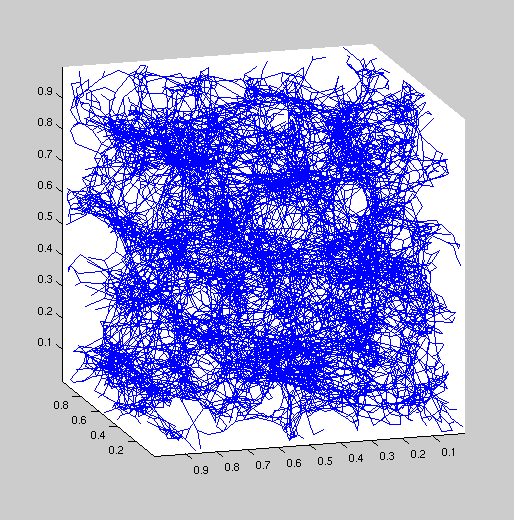
\includegraphics[width=0.92\textwidth]{Figures/chapter-reconstruct/networkN10000.png}%
    \label{collagen_network}
  \end{subfigure}%
  \begin{subfigure}{0.5\textwidth}
    \centering
    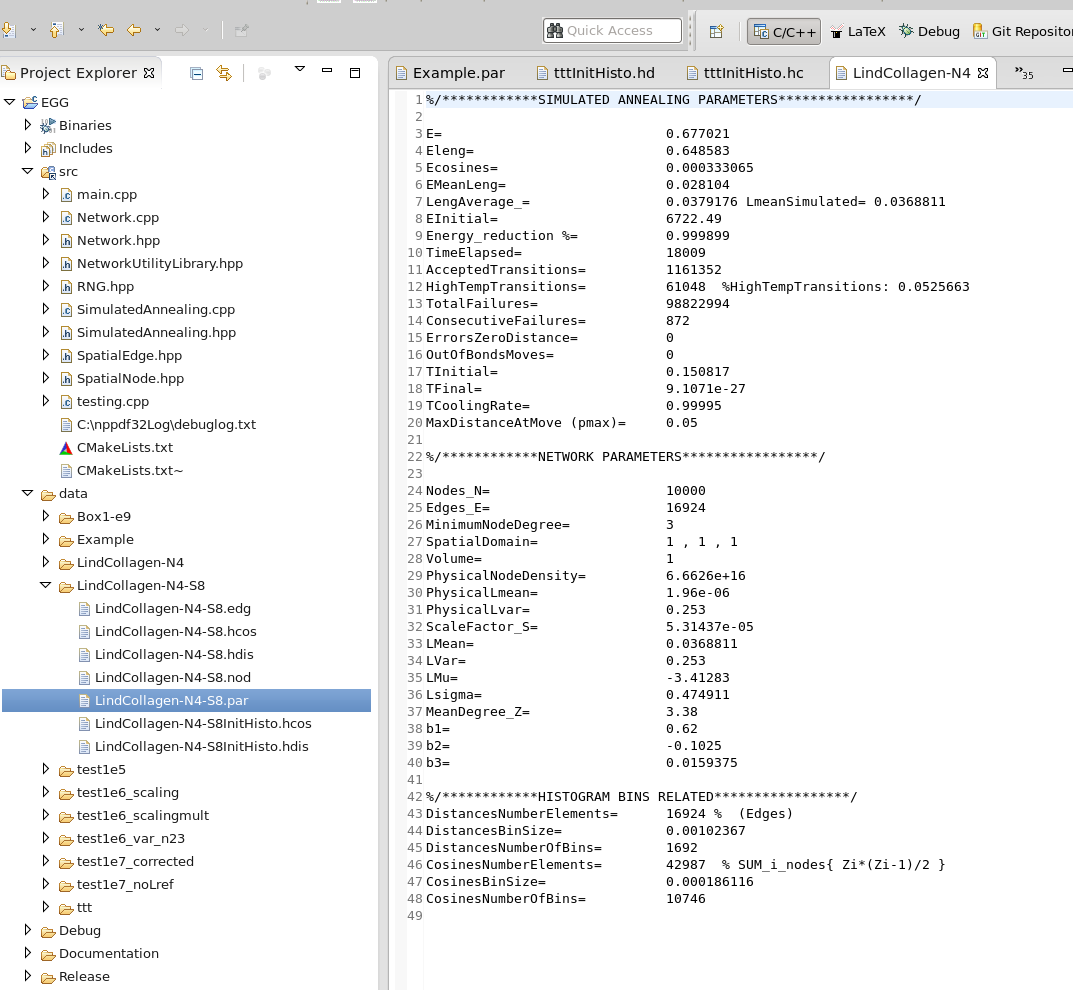
\includegraphics[width=0.92\textwidth]{Figures/chapter-reconstruct/parametersN10000.png}%
    \label{collagen_param}
  \end{subfigure}

\caption[Testing with theoretical collagen data]{ Reconstructed collagen
network \subref{collagen_network} Visualization of reconstructed collagen
network using Matlab. \subref{collagen_param} Simulation parameters from the reconstruction
algorithm.}
\label{fig:collagen-network}
\end{figure}



\begin{figure}[h!]
  \centering
  \begin{subfigure}{0.7\textwidth}
    \centering
    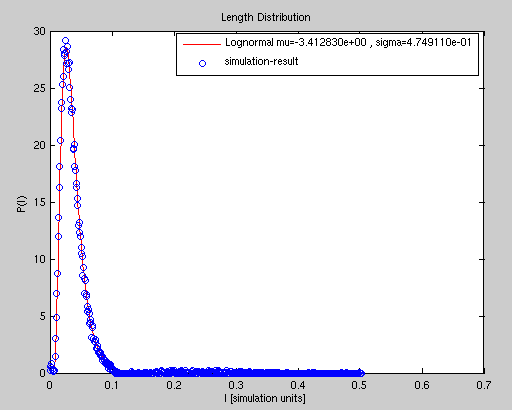
\includegraphics[width=0.92\textwidth]{Figures/chapter-reconstruct/lengthN10000.png}%
    \label{collagen_length}
  \end{subfigure}\\[1ex]
  \begin{subfigure}{0.7\textwidth}
    \centering
    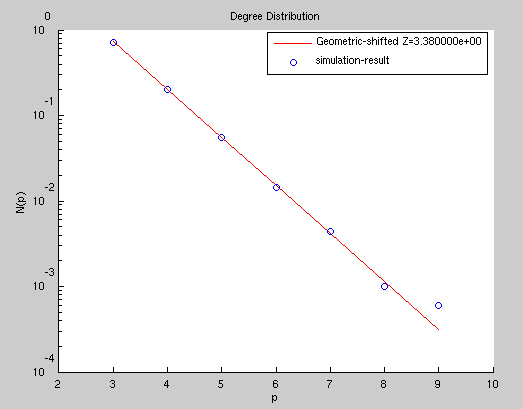
\includegraphics[width=0.92\textwidth]{Figures/chapter-reconstruct/degreeN10000.png}%
    \label{collagen_degree}
  \end{subfigure}\\[1ex]
  \begin{subfigure}{0.7\textwidth}
    \centering
    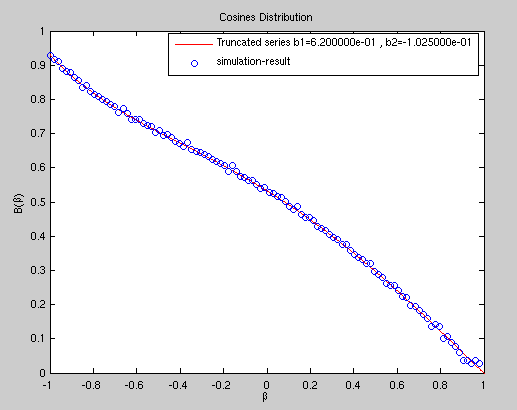
\includegraphics[width=0.92\textwidth]{Figures/chapter-reconstruct/cosinesN10000.png}%
    \label{collagen_cosines}
  \end{subfigure}

\caption[Collagen: comparing target and simulated distributions]{ Comparison
between target distributions and simulated results in the reconstructed collagen
network.
\subref{collagen_length} Length Distribution $P(\ell)$.
\subref{collagen_degree} Degree distribution $N(p)$.
\subref{collagen_cosines} Direction cosines distribution $B(\beta)$.
}
\label{fig:collagen-distributions}
\end{figure}

% \subsection{Actin data}
% The real use of the algorithm will be to reconstruct networks with different
% statistical distribution. These statistics will be gathered from image analysis,
% but also we can input any statistical distribution ``engineered'' by us, to
% study the generated network architecture.
%
% The image analysis of our data (chapter.\ref{Chapter-Image}) generates the
% needed input for the reconstruction algorithm, i.e. the statistical
% distributions of length, degree, and direction cosines.
% The length and degree distributions of actin data seems to follow (with both
% image analysis methods) a log-normal and geometrical distribution respectively.
% These are the same distributions proposed by Lindstrom for collagen (changing the parameters). But actin seems to
% follow a different distribution for direction cosines, (see
% Fig.\ref{fig:avizo_histograms30}) at least with the image analysis resulted from
% Avizo.  I am currently working on a way to extract the cosines distributions
% from FIRE algorithm to compare it.
%
%  When we will have the parameters of the cosines distributions of actin, we
% can easily implement it in the reconstruct software, and then generate
% the network following those distributions.
%
% The step in the future is to study the relation of the network architecture to
% mechanical properties and dynamics of the network.
